\section{Giá trị lớn nhất và nhỏ nhất của hàm số}
\subsection{Đề 1}
\Opensolutionfile{ans}[ans/ans-2-B2-De1-lc]
\caulc
\begin{ex}%[2D1N3-1]
	Tìm giá trị nhỏ nhất của hàm số $y=\dfrac{x+3}{x-1}$ trên đoạn $[-1;0]$.
	\choice
	{\True $\displaystyle\min\limits_{[-1;0]}y=-3$}
	{$\displaystyle\min\limits_{[-1;0]}y=-2$}
	{$\displaystyle\min\limits_{[-1;0]}y=-4$}
	{$\displaystyle\min\limits_{[-1;0]}y=3$}
	\loigiai{Hàm số $y=\dfrac{x+3}{x-1}$ xác định trên đoạn $[-1;0]$, có $y'=\dfrac{-4}{(x-1)^2}<0$  $\forall x\in [-1;0]$.\\ $\min\limits_{[-1;0]} y=y(0)=-3$.}
\end{ex}
\begin{ex}%[2D1N3-2]
	\immini{Giá trị nhỏ nhất trên tập xác định của hàm số có đồ thị sau là 		
		\choice
		{\True $\min\limits_{\mathscr{D}} y=-1$}
		{$\min\limits_{\mathscr{D}} y=1$}
		{$\min\limits_{\mathscr{D}} y=0$}
		{$\min\limits_{\mathscr{D}} y=-2$}}
	{
		{\color{black} 
			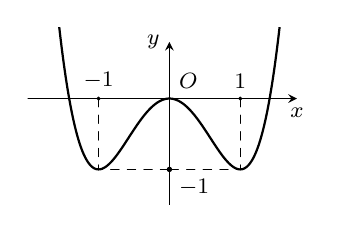
\begin{tikzpicture}[scale=0.9,>=stealth, font=\footnotesize, line join=round, line cap=round]
				%	\draw[color=gray!50,dashed] (-4,-6) grid (4,5);
				\clip (-2,-1.5) rectangle (2,1);
				\draw[->] (-2,0)--(1.8,0) node [below]{$x$};
				\draw[->] (0,-1.5)--(0,0.8) node [left]{$y$};
				\draw[samples=300,thick,domain=-1.7:1.7]plot(\x,{(\x)^4-2*(\x)^2});
				\draw [dashed](-1,0)|-(-1,-1)|-(0,-1);
				\draw [dashed](1,0)|-(1,-1)|-(0,-1);
				\draw node at(-1,0)[above]{$-1$};
				\draw node at (1,0)[above]{$1$};
				\draw node at (0,0)[above right]{$O$};
				\draw node at (0,-1)[below right]{$-1$};
				\draw[fill=black](-1,0)circle(0.2mm);
				\draw[fill=black](1,0)circle(0.2mm);
				\draw[fill=black](0,-1)circle(0.3mm);
	\end{tikzpicture}}}
	\loigiai{Giá trị nhỏ nhất bằng $-1$.}
\end{ex}
\begin{ex}%[2D1N3-1]
	Tìm giá trị lớn nhất của hàm số $f(x)=x^3-2x^2-4x+1$ trên đoạn $[ 1;3 ]$.
	\choice 
	{$\max\limits_{[1;3]}f( x )=-7$}
	{$\max\limits_{[1;3]}f( x )=-4$}
	{\True $\max\limits_{[1;3]}f( x )=-2$}
	{$\max\limits_{[1;3]}f( x )=-\dfrac{67}{27}$}
	\loigiai
	{
		Ta có $f'(x)= 3 x^{2}- 4 x - 4 , f'(x)= 0 \Leftrightarrow \hoac{& x = 2&&\text{(nhận)}\\ & x = - \dfrac{2}{3}&&\text{(loại)}.}$\\
		Ta tính $f(1)= - 4 , f(2)= - 7 , f(3)= - 2$ nên $\max\limits_{[1;3]} f(x)=-2$.
	}
\end{ex}
\begin{ex}%[2D1N1-1]
	Giá trị lớn nhất của hàm số $y=\dfrac{x+1}{x-2}$ trên $\left[-1;0\right]$	là
	\choice
	{$-\dfrac{1}{2}$ }
	{ $-\dfrac{2}{3}$}
	{ $2$}
	{ \True $0$}
	\loigiai{
		Hàm số $y=\dfrac{x+1}{x-2}$	 xác định và liên tục trên $\left[-1;0\right]$ có
		$y'=\dfrac{-3}{(x-2)^2}<0, \, \forall x \in \left[-1;0\right] $. Suy ra hàm số nghịch biến trên $\left[-1;0\right]$.\\
		Do đó, $\max \limits_{\left[-1;0\right] } y = y(-1) = 0$.
	}
\end{ex}
\begin{ex}%[2D1H3-1]
	Cho hàm số $f(x)=-2 x^{4}+4 x^{2}+10$. Tìm giá trị lớn nhất $M$ và giá trị nhỏ nhất $m$ của hàm số trên đoạn $[0 ; 2]$.
	\choice
	{ $M=10 ; m=-6$}
	{\True$M=12 ; m=-6$}
	{ $M=10 ; m=-8$}
	{$M=12 ; m=-8$}
	\loigiai{
		Ta có $f'(x)=-8x^3+8x; f'(x)=0 \Leftrightarrow \hoac{x=0 \in [0 ; 2]\\ x=1\in [0; 2]\\ x=-1 \notin [0; 2] } $;
		$\heva{&f(0)=10\\ &f(1)=12\\ &f(2)=-6}\Rightarrow  \heva{M=12\\m=-6.}$
	}
\end{ex}
\begin{ex}%[2D1H3-2]
	Giá trị lớn nhất của hàm số $y=\sqrt{x+2}-x$ là
	\choice
	{$-\dfrac{5}{4}$}
	{$\sqrt{3}-1$}
	{\True $\dfrac{9}{4}$}
	{$2$}
	\loigiai{
		Tập xác định $\mathscr{D}=[-2;+\infty), y' =\dfrac{1}{2\sqrt{x+2}}-1\Rightarrow y'=0\Leftrightarrow x=-\dfrac{7}{4}$.\\
		Bảng biến thiên
		\begin{center}
			
\begin{tikzpicture}[scale=1, line join=round, line cap=round]
				\tkzTabInit[nocadre=false,lgt=1,espcl=2.5]
				{$x$ /1,$y'$ /0.8,$y$ /2}
				{$-2$,$-\dfrac{7}{4}$,$+\infty$}
				\tkzTabLine{,+,$0$,-,}
				\tkzTabVar{-/$2$, +/$\dfrac{9}{4}$,-/$-\infty$}
			\end{tikzpicture}
		\end{center}
		Từ bảng biến thiên ta có $\max\limits_{\mathscr{D}} y=\dfrac{9}{4}$.
	}
\end{ex}
\begin{ex}%[2D1H3-2]
Tìm giá trị lớn nhất $M$ của hàm số $y=-2\sqrt{4-x}$.
\choice
{$M=-4$}
{$M=-2$}
{$M=1$}
{\True $M=0$}
\loigiai{
	Điều kiện: $4-x\leq 0 \Leftrightarrow x\leq 4$. \\
	Ta có $y=-2\sqrt{4-x}\leq 0$, $\forall x\leq 4$. Đẳng thức xảy ra khi $x=4$.
	Do đó $M=\max\limits_{(-\infty;4]}y=0$.}
\end{ex}
\begin{ex}%[2D1H3-2]
	Tìm giá trị lớn nhất $M$ của hàm số $y=\dfrac{x+1}{\sqrt{x^2+1}}$ trên khoảng $\left( {-\infty;+\infty} \right)$.
	\choice
	{$M=2\sqrt{2}$}
	{$M=1$}
	{\True $M=\sqrt{2}$}
	{$M=2$}
	\loigiai{
		Ta có $y'=0 \Leftrightarrow \dfrac{1-x}{\left( {x^2+1} \right)\sqrt{x^2+1}}=0 \Leftrightarrow x=1$.
		\\Bảng biến thiên
		\begin{center}
			
\begin{tikzpicture}[scale=0.8]
				\tkzTabInit
				[lgt=3,espcl=3] % tùy chọn
				{$x$/1.2, $y'$/1, $y$/2.5} % cột đầu tiên
				{$-\infty$, $1$, $+\infty$} % hàng 1 cột 2
				\tkzTabLine{,+,0,-,} % hàng 2 cột 2
				\tkzTabVar{-/ $-1$, +/ $\sqrt{2}$ , -/ $1$} % hàng 3 cột 2
			\end{tikzpicture}
		\end{center}
		Dựa vào bảng biến thiên ta thấy giá trị lớn nhất của hàm số là $M=\sqrt{2}$.}
\end{ex}
\begin{ex}%[2D1H3-2]
	Giá trị lớn nhất của hàm số $y = 2x + \dfrac{1}{x}$ khi $x < 0$ là
	\choice
	{$2\sqrt{2}$}
	{\True $-2\sqrt{2}$}
	{Không tồn tại}
	{$4$}
	\loigiai{
		Với $x < 0$, ta có $y = 2x + \dfrac{1}{x} = -\left[2(-x) + \dfrac{1}{-x}\right] \leq -2\sqrt{2(-x)\cdot\dfrac{1}{-x}} = -2\sqrt{2}$.\\
		Vậy giá trị lớn nhất của hàm số $y = 2x + \dfrac{1}{x}$ khi $x < 0$ là $-2\sqrt{2}$.
	}
\end{ex}
\begin{ex}%[2D1H3-2]
	Giá trị lớn nhất của hàm số $f(x)=x(1-x^2)$ trên khoảng $(0;1)$ là
	\choice
	{$\dfrac{1}{9}$}
	{$\dfrac{1}{\sqrt{3}}$}
	{$0$}
	{\True $\dfrac{2\sqrt{3}}{9}$}
	\loigiai{
		Xét trên $(0;1)$. Ta có\\
		$f'(x)=-3x^2+1$.\\
		$f'(x)=0\Leftrightarrow x=\pm \dfrac{1}{\sqrt{3}} \in (0;1)$.\\
		Hàm số $y=f(x)$ liên tục trên $(0;1)$, đồng thời
		$\lim\limits_{x\to 0^+}f(x)=0$; $f\left(\dfrac{1}{\sqrt{3}}\right)=\dfrac{2\sqrt{3}}{9}$; $f\left(-\dfrac{1}{\sqrt{3}}\right)=-\dfrac{2\sqrt{3}}{9}$; $\lim\limits_{x\to 1^-}f(x)=0$.\\
		Vậy $\max\limits_{(0;1)} f(x)=\dfrac{2\sqrt{3}}{9}$.
	}
\end{ex}
\begin{ex}%[2D1V3-2]
	Cho hàm số $y=f(x)$ có đạo hàm cấp hai trên $\mathbb{R}$. Biết $f'(0)=3$, $f'(2)=-2$ và bảng xét dấu của $f''(x)$ như sau
	\begin{center}
		
\begin{tikzpicture}
			\tkzTabInit[nocadre=false,lgt=1.2,espcl=2.5]
			{$x$ /0.6,$f''(x)$ /0.6}
			{$-\infty$,$0$,$2$,$+\infty$}
			\tkzTabLine{,+,$0$,-,$0$,+,}
		\end{tikzpicture}
	\end{center}
	Hàm số $y=f(x+3)+2x$ đạt giá trị nhỏ nhất tại điểm $x_0$ thuộc khoảng nào sau đây?
	\choice
	{$(3;+\infty)$}
	{\True $(-\infty;-3)$}
	{$(0;3)$}
	{$(-2;0)$}
	\loigiai{
		Từ bảng xét dấu của $f''(x)$ ta có bảng biến thiên của $f'(x)$ như sau
		\begin{center}
			
\begin{tikzpicture}
				\tkzTabInit[nocadre=false,lgt=2,espcl=2.5]
				{$x$ /0.6,$f''(x)$ /0.6,$f'(x)$ /2,$f'(x)+2$/2}
				{$-\infty$,$0$,$2$,$+\infty$}
				\tkzTabLine{,+,$0$,-,$0$,+,}
				\tkzTabVar{-/$-\infty$, +/$3$,-/$-2$,+/$+\infty$}
				\tkzTabVar{-/$-\infty$, +/$5$,-/$0$,+/$+\infty$}
			\end{tikzpicture}
		\end{center}
	Từ BBT, ta thấy $f'(x)+2=0\Leftrightarrow \hoac{&x=2\\&x=a<0.}$\\
	Ta có BBT của $y=f(x)+2x$ như sau
		\begin{center}
		
\begin{tikzpicture}
			\tkzTabInit[nocadre=false,lgt=2,espcl=2.5]
			{$x$ /0.6,$f'(x)+2$ /0.6,$f(x)+2x$ /2}
			{$-\infty$,$a$,$2$,$+\infty$}
			\tkzTabLine{,-,$0$,+,$0$,+,}
			\tkzTabVar{+/$+\infty$, -/$f(a)+2a$,R,+/$+\infty$}
		\end{tikzpicture}
	\end{center}
	Từ BBT, ta thấy hàm số $y=f(x)+2x$ đạt GTNN tại $x=a, (a<0)$.\\
	Vậy hàm số $y=f(x+3)+2x$ đạt GTNN tại $x=a-3$.
	}
\end{ex}
\begin{ex}%[2D1V3-1]
	Xét hàm số 	$f(x)=\left|x^2 + a x + b\right|$, với $a$, $b$ là tham số. Gọi $M$ là giá trị lớn nhất của hàm số trên $[-1;3]$. Khi đó $M$ nhận giá trị nhỏ nhất có thể được, tính $a+2b$.
	\choice
	{$3$}
	{$4$}
	{\True $-4$}
	{$2$}
	\loigiai{
		Ta có $\heva{& M \geq|f(-1)|=|b-a+1|; \; M \geq|f(3)|=|b+3 a+9| \quad &(1)\\& M \geq|f(1)|=|b+a+1| \Rightarrow 2 M \geq|-2 b-2 a-2| &(2). }$\\
		Từ $(1)$ và $(2)$, kết hợp với 	$|x| + |y| + |z|\geq|x + y + z|$, ta được
		\begin{eqnarray*}
			4M & \ge & |b-a+1|+|b+3 a+9|+|-2 b-2 a-2| \\
			& \ge & |b-a+1+b+3 a+9-2 b-2 a-2|=8.
		\end{eqnarray*}	
		Suy ra $M \ge 2$.\\
		Dấu \lq \lq $=$\rq \rq \, xảy ra khi $\heva{&|b-a+1|=2\\ & |b+3 a+9|=2\\ &|b+a+1|=2 }$ và $b-a+1$, $b+3a+9$, $-2a-2a-2$ cùng dấu.\\
		Do đó $\heva{&a=-2\\&b=-1} \Rightarrow a+2b=-4$.
	}
\end{ex}
\Closesolutionfile{ans}
\indapan{6}{ans/ans-2-B2-De1-lc}
\Opensolutionfile{ans}[ans/ans-2-B2-De1-ds]
\cauds
\setcounter{ex}{0}
\begin{ex}%[2D1H3-1]
	\immini
	{Hàm số $y=f(x)$ liên tục trên đoạn $[-1;3]$ và có bảng biến thiên như sau. Gọi $M$ và $m$ lần lượt là GTLN và GTNN của hàm số trên $[-1;3]$. Khẳng định nào đúng?
		\choiceTF
		{$m=f(2)$}
		{$M=f(4)$}
		{\True $m=f(-1)$}
		{\True $M=f(0)$}}
	{
\begin{tikzpicture}
			\tkzTabInit[nocadre=false,lgt=1.2,espcl=2]
			{$x$ /0.8,$y'$ /0.8,$y$ /2}
			{$-1$,$0$,$2$,$3$}
			\tkzTabLine{,+,$0$,-,$0$,+,}
			\tkzTabVar{-/$0$, +/$5$,-/$1$,+/$4$}
	\end{tikzpicture}}
	\loigiai
	{Dựa vào bảng biến thiên ta có $M=f(0)=5$ và $m=f(-1)=0$.}
\end{ex}
\begin{ex}%[2D1H3-1]
	Tìm khẳng định đúng. Xét trên khoảng $(-\infty;+\infty)$, hàm số $y=x^4+2x^2-3$
	\choiceTF
	{không có cả giá trị lớn nhất và nhỏ nhất}
	{\True có cực trị}
	{\True có giá trị nhỏ nhất}
	{có giá trị lớn nhất}
	\loigiai
	{
			Tập xác định: $\mathscr{D}=\mathbb{R}$.\\
		$y'=4x^3+6x=2x(x^2+3)$.\\
		$y'=0\Leftrightarrow x=0$.\\
		Bảng biến thiên:
		\begin{center}
			
\begin{tikzpicture}[>=stealth,scale=1]
				\tkzTabInit[lgt=1.2,espcl=4]
				{$x$/1,$y'$/1,$y$/2}
				{$-\infty$,$0$,$+\infty$}
				\tkzTabLine{ ,-,0,+, }
				\tkzTabVar {+/$+\infty$,-/$-3$,+/$+\infty$}
			\end{tikzpicture}
		\end{center}
		Vậy hàm số có giá trị nhỏ nhất là $-3$ khi $x=0$, có cực trị và không có giá trị lớn nhất.}
\end{ex}
\begin{ex}%[2D1H3-2]
	\immini{Cho hàm số $y=f(x)$ liên tục trên $\mathbb{R}$ và có đồ thị như hình dưới đây. Mệnh đề nào đúng?
	\choiceTF
	{\True Hàm số nghịch biến trên khoảng $(0;1)$}
	{Hàm số đồng biến trên khoảng $(-1;2)$}
	{\True Hàm số có ba điểm cực trị}
	{Hàm số có giá trị lớn nhất bằng $2$}
	}{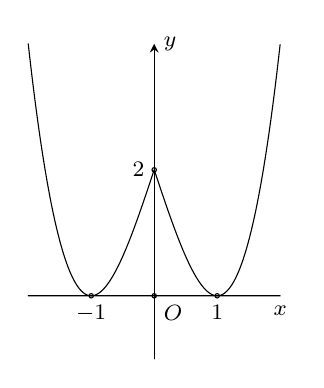
\begin{tikzpicture}[scale=0.8, font=\footnotesize, line join=round, line join=round, line cap = round,>=stealth]
			\draw[->] (-2,0)--(0,0) node[below right]{$O$} circle (1pt)--(2,0) node[below]{$x$};
			\draw[->] (0,-1) --(0,4) node[right]{$y$};
			\foreach \x in {-1,1}{
				\draw (\x,0) node[below]{$\x$} circle (1pt);}
			\foreach \y in {2}{
				\draw (0,\y) node[left]{$\y$} circle (1pt);}
			\draw [domain=0:2, samples=100] %
			plot (\x, {(\x)^3-3*(\x)+2});
			\draw [domain=-2:0, samples=100] %
			plot (\x, {-(\x)^3+3*(\x)+2});
		\end{tikzpicture}
	}
	\loigiai{
		Dựa vào đồ thị hàm số, ta thấy
		\begin{itemchoice}
		\itemch Hàm số nghịch biến trên khoảng $(0;1)$ là khẳng định đúng.
		\itemch Hàm số đồng biến trên khoảng $(-1;2)$ là khẳng định sai, vì trên khoảng $(0;1)$ hàm số nghịch biến.
		\itemch Hàm số có ba điểm cực trị là khẳng định đúng, hàm số có $3$ điểm cực trị tại $x=-1$, $x=0$, $x=1$.
		\itemch Hàm số có giá trị lớn nhất bằng $2$ là khẳng định sai, hàm số có giá trị cực đại bằng $2$, không tồn tại giá trị lớn nhất.
		\end{itemchoice}
	}
\end{ex}
\begin{ex}%[2D1V3-2]
	Cho hàm số $y=f\left(x\right)$ xác định và liên tục trên khoảng $(-3;2)$ có $\lim\limits_{x\to\left(-3\right)^+}f\left(x\right)=-5$, $\lim\limits_{x\to2^-}f\left(x\right)=3$ và có bảng biến thiên như sau
	\begin{center}
		
\begin{tikzpicture}
			\tkzTabInit[lgt=1.2,espcl=2.5,deltacl=0.6]
			{$x$/0.6,$y'$/0.6,$y$/2}
			{$-3$,$-1$,$1$,$2$}
			\tkzTabLine{,+,0,-,0,+,}
			\tkzTabVar{-/$-5$,+/$0$,-/$-2$,+/$3$}
		\end{tikzpicture}
	\end{center}
	Mệnh đề nào dưới đây đúng?
	\choiceTF
	{\True Hàm số không có giá trị nhỏ nhất trên khoảng $\left(-3;2\right)$}
	{\True Giá trị cực đại của hàm số bằng $0$}
	{Giá trị lớn nhất của hàm số trên khoảng $\left(-3;2\right)$ bằng $0$}
	{\True Giá trị cực tiểu của hàm số bằng $-2$}
	\loigiai{
		Dựa vào bảng biến thiên, hàm số không đạt giá trị lớn nhất trên $ (-3;2) $.
	}
\end{ex}
\Closesolutionfile{ans}
\indapan{3}{ans/ans-2-B2-De1-ds}
\Opensolutionfile{ans}[ans/ans-2-B2-De1-kq]
\caukq
\setcounter{ex}{0}
\begin{ex}%[2D1H3-1]
	\immini{
		Cho hàm số $y=f(x)$ liên tục trên đoạn $[-1;3]$ và có đồ thị như hình vẽ bên. Gọi $M,m$ lần lượt là giá trị lớn nhất và giá trị nhỏ nhất của hàm số đã cho trên đoạn $[-1;3]$. Tính $M-m$.
	}{
		\begin{tikzpicture}[scale=1, font=\footnotesize, line join=round, line cap=round,>=stealth]
			\def\xmin{-1.5} \def\xmax{4}
			\def\ymin{-3.5} \def\ymax{3}
			\clip (\xmin+0.1,\ymin+0.1) rectangle (\xmax-0.1,\ymax-0.1);
			%	\tkzInit[xmin=-1.5, xmax=4, ymin=-3.5, ymax=3]
			%	\tkzClip
			\draw[->] (-1.5,0) -- (-1,0) node[above]{$-1$} -- (0,0) node[below left]{$O$} -- (2,0) node[below]{$2$} -- (3,0) node[above]{$3$} -- (3.5,0) node[below]{$x$};
			\draw[->] (0,-3.5) -- (0,-3) node[below left]{$-3$} -- (0,-2) node[below left]{$-2$} -- (0,-1) node[below left]{$-1$} -- (0,2) node[left]{$2$} -- (0,2.7) node[right]{$y$};
			\draw[dashed] (-1,0) -- (-1,-1) -- (0,-1) (0,2) -- (2,2) -- (2,0) (3,0) -- (3,-3) -- (0,-3);
			\draw [black, domain=-1:2, samples=100] plot (\x, {(\x)^2-2});
			\draw [black, domain=2:3, samples=100] plot (\x, {12-5*(\x)});
		\end{tikzpicture}
	}
	\shortans{$5$}
	\loigiai{
		Dựa vào đồ thị ta có $M=\max\limits_{[-1;3]}f(x)=f(2)=2$ và $m=\min\limits_{[-1;3]}f(x)=f(3)=-3$ nên $M-m=5$.
	}
\end{ex}
\begin{ex}%[2D1H3-1]
	Biết hàm số $y=x^3-3x^2-9x+28$ đạt giá trị nhỏ nhất trên đoạn $[0;4]$ tại $x_0$. Tính $P=x_0+2$.
	\shortans{$5$}
	\loigiai{Ta có $y'=3x^2-6x-9=0\Leftrightarrow \hoac{&x=3\\&x=-1 \,\, \text{(loại)}.}$\\
		Khi đó $y(0)=28$, $y(3)=1$, $y(4)=8$.\\
		 Do đó $\min\limits_{x\in[0;4]} f(x)=\min\{y(0), y(3), y(4)\}=1$ tại $x_0=3$.
		\\ Vậy $P=3+2=5$.
	}
\end{ex}
\begin{ex}%[2D1V3-1]
	Tìm $m$ để hàm số $y=\dfrac{x-m}{mx+1}$ có giá trị nhỏ nhất trên $[0;1]$ bằng $-2$.
		\shortans{$2$}
	\loigiai{
		\begin{itemize}
			\item Nếu $m=0$ thì hàm số đã cho trở thành $y=x$ có giá trị nhỏ nhất trên $[0;1]$ bằng $0$ (không thỏa mãn yêu cầu bài toán).
		\item Nếu $m \neq 0$ thì hàm số đã cho xác định khi $x\neq -\dfrac{1}{m}$.\\
		Ta có $y'=\dfrac{m^2+1}{(mx+1)^2}>0, \forall x \neq -\dfrac{1}{m}$ nên hàm số đã cho luôn đồng biến trên mỗi khoảng xác định của nó.\\
		Hàm số đã cho có giá trị nhỏ nhất trên $[0;1]$ bằng $-2$ khi
		\[\heva{&\hoac{&-\dfrac{1}{m}<0 \\&-\dfrac{1}{m}>1} \\&y(0)=-2} \Leftrightarrow \heva{&\hoac{&m>0 \\&-1<m<0} \\&-m=-2} \Leftrightarrow m=2.\]
	\end{itemize}
	}
\end{ex}
\begin{ex}%[2D1V3-1]
	Tìm $m$ để hàm số $y=\dfrac{x-m}{mx+1}$ có giá trị nhỏ nhất trên $[0;1]$ bằng $-2$.
	\shortans{$2$}
	\loigiai
	{
		Nếu $m=0$ thì hàm số đã cho trở thành $y=x$ có giá trị nhỏ nhất trên $[0;1]$ bằng $0$ (không thỏa mãn yêu cầu bài toán).\\
		Nếu $m \neq 0$ thì hàm số đã cho xác định khi $x\neq -\dfrac{1}{m}$.\\
		Ta có $y'=\dfrac{m^2+1}{(mx+1)^2}>0, \forall x \neq -\dfrac{1}{m}$ nên hàm số đã cho luôn đồng biến trên mỗi khoảng xác định của nó.\\
		Hàm số đã cho có giá trị nhỏ nhất trên $[0;1]$ bằng $-2$ khi
		\[\heva{&\hoac{&-\dfrac{1}{m}<0 \\&-\dfrac{1}{m}>1} \\&y(0)=-2} \Leftrightarrow \heva{&\hoac{&m>0 \\&-1<m<0} \\&-m=-2} \Leftrightarrow m=2.\]
	}
\end{ex}
\begin{ex}%[2D1C3-6]
	Một xưởng in có $8$ máy in, mỗi máy in được $3\;600$ bản in trong một giờ. Chi phí để vận hành một máy in trong mỗi lần in là $50$ nghìn đồng. Chi phí cho $n$ máy in chạy trong một giờ là $60(6n+10)$ nghìn đồng. Hỏi nếu in $50\;000$ tờ quảng cáo thì phải sử dụng bao nhiêu máy in để được lãi nhiều nhất?	
	\shortans{$5$}
	\loigiai
	{Một máy trong một giờ in được $3\;600$ tờ nên $50\;000$ tờ cần $\dfrac{125}{9}$ giờ.\\
		Do đó $n$ máy cần thời gian là $\dfrac{125}{9n}$ giờ.\\
		Tổng chi phí là $f(n)=\left[10\cdot \left(6n+10\right)\right]\cdot 1000+50\;000n$.\\
		Khi đó, để lãi nhiều nhất thì $f(n)$ đạt giá trị nhỏ nhất, với $n\in \left[1;8\right]$ và $n\in \mathbb{N}$.\\
		Cách 1: $f(n)=\left(\dfrac{250}{3}+\dfrac{1250}{9n}+5n\right)\cdot 10000\geq \left(\dfrac{250}{3}+\dfrac{50\sqrt{10}}{3}\right)$ (BĐT AM - GM).\\
		Do đó, $f(n)$ nhỏ nhất khi $\dfrac{1250}{9n}=4n\Leftrightarrow n =\dfrac{5\sqrt{5}}{10}\approx 5$.\\
		Cách 2: Dùng Table lập bảng $f(n)$ với $n\in \left\{1; 2; \ldots ; 8\right\}$ từ đó suy ra $n=5$.  
	}
\end{ex}
\begin{ex}%[2D1C3-6]
	Ông An muốn xây một cái bể chứa nước lớn dạng một khối hộp chữ nhật không nắp có thể tích bằng $288 \mathrm{\, m^3}$. Đáy bể là hình chữ nhật có chiều dài gấp đôi chiều rộng, giá thuê nhân công để xây bể là $500\;000$ đồng/$\mathrm{m^2}$. Nếu ông An biết xác định các kích thước của bể hợp lí thì chi phí thuê nhân công sẽ thấp nhất. Hỏi ông An trả chi phí thấp nhất để xây dựng bể đó là bao nhiêu? (Đơn vị: triệu đồng)
	\shortans{$108$}
	\loigiai{
		Theo bài ra ta có để chi phí thuê nhân công là thấp nhất thì ta phải xây dựng bể sao cho tổng diện tích xung quanh và diện tích đáy là nhỏ nhất.\\
		Gọi ba kích thước của bể là $a \mathrm{\, m}$, $2a \mathrm{\, m}$, $c \mathrm{\, m}$ (với $a>0$, $c>0$).\\
		Ta có diện tích các mặt cần xây là $S= 2a^2+ 4ac+ 2ac= 2a^2+ 6ac$.\\
		Thể tích bể là $V= a\cdot 2a\cdot c= 2a^2c= 288\Rightarrow c= \dfrac{144}{a^2}$.\\
		Do đó $S= 2a^2+ 6a\cdot \dfrac{144}{a^2}= 2a^2+ \dfrac{864}{a}= 2a^2+ \dfrac{432}{a}+ \dfrac{432}{a}\ge 3\sqrt[3]{2a^2\cdot \dfrac{432}{a}\cdot \dfrac{432}{a}}= 216$.\\
		Vậy chi phí thấp nhất để xây dựng bể là $216\times 500000= 108$ triệu đồng.
	}
\end{ex}
\Closesolutionfile{ans}
\indapan{6}{ans/ans-2-B2-De1-kq}